
\section{Tight Binding Theory}

\subsection{Energy Band Structure}

An important concept in quantum mechanics and solid state physics is the band structure of solids. All atoms have a particular electron configuration, which characterises its quantum mechanical and electronic properties. Sodium ($\mathrm{Na}$), for instance, has atomic number $Z=11$ and therefore eleven electrons \cite{Quinn2018}. Four of these electrons fill the $1s$ and the $2s$ shell, six more fill the $2p$ shell and one electron occupies the $3s$ shell. The $1s$, $2s$ and $2p$ shells are closed whereas the last electron in the $3s$ configuration is a valence electron, which is responsible for bonding to other atoms or molecules. Another important group of electrons are the conduction electrons (in the case of $\mathrm{Na}$ this is the $3s$ electron), which are responsible for the conductivity of a solid.

\begin{figure}[H]
    \centering
    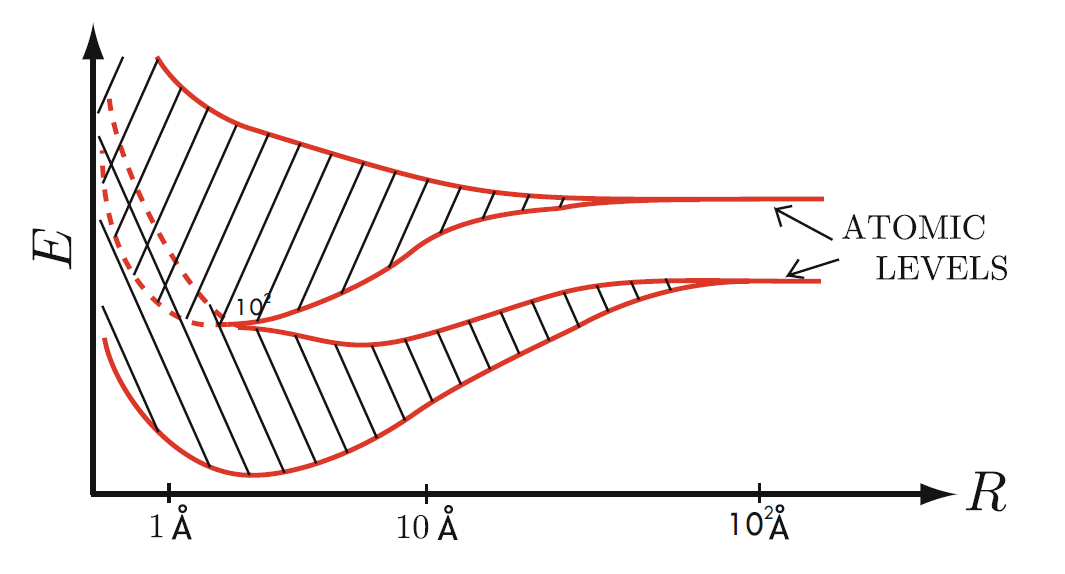
\includegraphics[width=.5\textwidth]{img/band_structure.PNG}
    \caption{Sketch of the band structure of a lattice at atomic energy level $E$ and interatomic distance $R$ \cite{Quinn2018} (image source: \textcite{Quinn2018}).}
    \label{fig:band_structure}
\end{figure}

Let us now consider two Sodium atoms separated by some distance $R$. If these atoms are brought closer together, they start experiencing the Coulomb potential from the other Sodium atom \cite{Quinn2018}. The Coulomb potentials of the two atoms start to overlap and the electrons in $\mathrm{Na}$ begin experiencing both potentials. As a consequence, the electron energy levels become degenerate, meaning that one energy level corresponds to several quantum mechanical states of this electron. This is an important effect in solids, where several atoms are packed closely to each other and form a lattice. If the nearest neighbour distance in these solids is decreased, the energy levels start to broaden and create energy bands, which can create an overlap (see figure \ref{fig:band_structure}) \cite{Quinn2018}. The valence electrons and the conduction electrons in a solid form the so-called valence and conduction bands. These bands represent the range of energy levels that electrons can occupy and ultimately determine with what kind of crystals we are dealing with (e.g. metals, semiconductors, insulators). In metals the conduction and valence bands overlap, while in semiconductors and insulators there are gaps between these bands. These overlaps and gaps define the electrical properties of these solids.

%%%%%%%%%%%%%%%%%%%%%%%%%%%%%%%%%

\subsection{Tight Binding Model}\label{tight_binding_method}

There are several methods to analyse energy bands in crystal structures. The two most well-known approximation methods are the tight binding model and the free electron model. The first model assumes that electrons have a rather strong bond to the ion core whereas the latter works with weakly bound electrons which do not experience a strong Coulomb repulsion (e.g. metals) \cite{Quinn2018}. In other words, the tight binding theory assumes that there is a strong periodic Coulomb potential which is an ideal model to describe covalently bound crystals, as the electrons in these solids experience a strong coupling \cite{Girvin2019, Hofmann2015}. Furthermore, the tight binding approximation can be used to describe the band structure of the lower shells too, because those electrons are tightly bound to the core \cite{Patterson2007}. It is important to point out that the free electron and the tight binding model are approximations and both of them can lead to good results for the band structure of a system if all contributing factors are considered \cite{Hofmann2015}. In this thesis we will be working with the tight binding approximation.

Suppose we have an atom with Coulomb potential $V_a(\mathbf{r})$ and a single valence electron (e.g. Sodium). The Schrödinger equation can then be written as \cite{Quinn2018}
\begin{equation}\label{eq:schrödinger}
    \brackets{-\frac{\hbar^2}{2m}\del^2+V_a(\mathbf{r})-E_a}\phi(\mathbf{r})=0,
\end{equation}
where $\hbar$ is the reduced Planck constant, $m$ the mass of the atom, $\del$ the del-operator, $E_a$ the atomic energy level and $\phi(\mathbf{r})$ the wave function of the electron with $\mathbf{r}$ representing the position of the electron relative to the core. If we are now dealing with a crystal in the tight binding theory, the Coulomb potential of each atom in the lattice overlaps with the potential of neighbouring atoms \cite{Quinn2018}. In the tight binding approximation we assume that only the nearest neighbours located at some point $\mathbf{R}_j$ contribute to this Coulomb potential. Due to the periodicity the energy of these neighbours can be assumed to be $E_a$ and the wave function can be written as $\phi(\mathbf{r-\mathbf{R}_j})$ \cite{Quinn2018}. Taking several of these points in a crystal lattice will create a linear combination\footnote{In some textbooks the tight binding method is sometimes referred to as the linear combination of atomic orbitals (LCAO) \cite{Patterson2007}.}. Furthermore from Bloch's theorem\footnote{Bloch's theorem states that a crystal with periodic boundary conditions meets the following condition: 
\begin{equation}
     \psi (\mathbf{r}) = e^{i \mathbf{k}\cdot\mathbf{r}}u_\mathbf{k}(\mathbf{r}),
\end{equation}
where $u_\mathbf{k}(\mathbf{r}) = u_\mathbf{k}(\mathbf{r}+\mathbf{a})$ is a periodic function (with periodicity $\mathbf{a}$) and $\mathbf{k}$ is the wave vector in momentum space \cite{Quinn2018}.} it follows that \cite{Quinn2018}
\begin{equation}\label{eq:psi}
\begin{split}
    &\psi_\mathbf{k}(\mathbf{r})=\frac{1}{\sqrt{N}}\sum_j e^{i \mathbf{k}\cdot\mathbf{r}}\phi\brackets{\mathbf{r}-\mathbf{R}_j}\\
    &\psi_\mathbf{k}(\mathbf{r}+\mathbf{R}_n)=e^{i \mathbf{k}\cdot\mathbf{R}_n}\psi_\mathbf{k}(\mathbf{r}).
\end{split}
\end{equation}
For the Band structure we have to find the energy of the state $\psi_\mathbf{k}(\mathbf{r})$ with Hamiltonian $H$, which in Dirac notation can be written as \cite{Quinn2018}
\begin{equation}\label{eq:E_k}
    E_\mathbf{k}=\frac{\dddirac{\psi_\mathbf{k}}{H}{\psi_\mathbf{k}}}{\ddirac{\psi_\mathbf{k}}{\psi_\mathbf{k}}}.
\end{equation}
The Hamiltonian is defined as the sum of the Coulomb potential and the kinetic energy of the electron \cite{Griffiths2018}. From equation \ref{eq:psi} it follows that \cite{Kittel2004}
\begin{equation}\label{eq:psi_H_psi}
    \dddirac{\psi_\mathbf{k}}{H}{\psi_\mathbf{k}} = \frac{1}{N}\sum_j\sum_me^{i\mathbf{k}\cdot(\mathbf{R}_j-\mathbf{R}_m)}\dddirac{\phi_m}{H}{\phi_j},
\end{equation}
where $\phi_m \equiv \phi(\mathbf{r}-\mathbf{R}_m)$ and $\phi_j \equiv \phi(\mathbf{r}-\mathbf{R}_j)$. By defining a new variable $\rho_m = \mathbf{R}_m - \mathbf{R}_j$, we can rewrite equation \ref{eq:psi_H_psi} as \cite{Kittel2004}
\begin{equation}\label{eq:int}
    \dddirac{\psi_\mathbf{k}}{H}{\psi_\mathbf{k}} = \sum_me^{i\mathbf{k}\cdot\rho_m} \int \dint^3 r \; \phi^*(\mathbf{r}-\rho_m)H\phi(\mathbf{r}).
\end{equation}
In many cases only the nearest neighbours at a distance $\rho$ and the on-site interaction has to be considered such that most integrals in equation \ref{eq:int} can be neglected, which implies that \cite{Kittel2004}
\begin{equation}
    \ddirac{\psi_\mathbf{k}}{\psi_\mathbf{k}} = 1,
\end{equation}
and
\begin{equation}
    \dddirac{\psi_\mathbf{k}}{H}{\psi_\mathbf{k}} = \int \dint^3 r \; \phi^*(\mathbf{r})H\phi(\mathbf{r})+ \int \dint^3 r \; \phi^*(\mathbf{r}-\rho)H\phi(\mathbf{r}) \sum_m\exp^{i\mathbf{k}\cdot\rho_m}.
\end{equation}
The energy of the state $\psi_\mathbf{k}(\mathbf{r})$ given in equation \ref{eq:E_k} can now be written as
\begin{equation}
    E_\mathbf{k} = -\alpha-\gamma \sum_m\exp^{i\mathbf{k}\cdot\rho_m},
\end{equation}
where $\alpha$ and $\gamma$ are defined as \cite{Kittel2004}
\begin{equation}
\begin{split}
    \alpha &= - \int \dint^3 r \; \phi^*(\mathbf{r})H\phi(\mathbf{r})\\
    \gamma &= - \int \dint^3 r \; \phi^*(\mathbf{r}-\rho)H\phi(\mathbf{r}).
\end{split}
\end{equation}
The band structure is now given by the energy $E_\mathbf{k}$ and the distance $\rho_m = \mathbf{R}_m - \mathbf{R}_j$ between two atoms. One can for instance easily determine the maximum and minimum value to find a bandwidth for $E_\mathbf{k}$ \cite{Quinn2018}.


\subsection{Tight Binding Model in the Second Quantisation Representation}\label{second_quant_repr}

Solid state physics often deals with many-body systems composed of interacting particles. The second quantisation method, originally designed by the English physicist Paul Dirac (1902 - 1984), offers an alternative to the Schrödinger formulation used in section \ref{tight_binding_method} \cite{Beale2020}. In the second quantisation the wave functions of the particles can be written in terms of the so-called annihilation and creation operators, which simplify the expression for the Hamiltonian. In our case it is convenient to define the following annihilation and creation operators respectively and their inverse \cite{Quinn2018}
\begin{equation}
\begin{split}
    c_n = \frac{1}{\sqrt{N}}\sum_\mathbf{k}c_\mathbf{k} e^{i\mathbf{k}\cdot\mathbf{R}_n^0} &\iff c_\mathbf{k} = \frac{1}{\sqrt{N}}\sum_n c_n e^{-i\mathbf{k}\cdot\mathbf{R}_n^0}\\
    c_n^\dagger = \frac{1}{\sqrt{N}}\sum_\mathbf{k}c_\mathbf{k}^\dagger e^{-i\mathbf{k}\cdot\mathbf{R}_n^0} &\iff c_\mathbf{k}^\dagger = \frac{1}{\sqrt{N}}\sum_n c_n e^{i\mathbf{k}\cdot\mathbf{R}_n^0}.
\end{split}
\end{equation}
The operator $c_n$ annihilates and $c_n^\dagger$ creates electrons at site $\mathbf{R}_n^0$. The kinetic energy of a system of electrons can then be written as \cite{Quinn2018}
\begin{equation}\label{eq:K}
\begin{split}
    K &= \sum_\mathbf{k}\epsilon_\mathbf{k}c_\mathbf{k}^\dagger c_\mathbf{k} =\frac{1}{N} \sum_\mathbf{k}\epsilon_\mathbf{k}\sum_{n,m}c_n^\dagger c_m e^{i\mathbf{k}\cdot\brackets{\mathbf{R}_n^0-\mathbf{R}_m^0}}\\
    &= \sum_{n,m}T_{n,m} c_n^\dagger c_m \where T_{n,m} \equiv \frac{1}{N}\sum_\mathbf{k}\epsilon_\mathbf{k}e^{i\mathbf{k}\cdot\brackets{\mathbf{R}_n^0-\mathbf{R}_m^0}}.
\end{split}
\end{equation}
$\epsilon_\mathbf{k}$ is the kinetic energy of a single electron with wave vector $\mathbf{k}$. The periodic potential can be written as a Fourier series of the form \cite{Quinn2018}
\begin{equation}\label{eq:V_r}
    V(\mathbf{r})=\sum_{\mathbf{K}} V_\mathbf{K}e^{i\mathbf{K}\cdot\mathbf{r}},
\end{equation}
where the sum over all wave vectors $\mathbf{K}$ form a lattice in reciprocal space. Note that this can only be done if the potential is periodic at each lattice point \cite{Quinn2018}. The potential energy of the electrons is then given by the relation \cite{Quinn2018}
\begin{equation}\label{eq:U}
\begin{split}
    U &= \sum_{\mathbf{k},\mathbf{K}}V_\mathbf{K}c_{\mathbf{k}+\mathbf{K}}^\dagger c_\mathbf{k} = \frac{1}{N} \sum_{\mathbf{k},\mathbf{K}}V_\mathbf{K} \sum_{n,m}c_n^\dagger e^{i(\mathbf{k}+\mathbf{K})\cdot\mathbf{R}_m^0}c_me^{-i\mathbf{k}\cdot\mathbf{R}_m^0}\\
    &= \frac{1}{N}\sum_{\mathbf{K},n,m}\underbrace{\abrackets{\sum_\mathbf{k}e^{i\mathbf{k}\cdot(\mathbf{R}_n^0-\mathbf{R}_m^0)}}}_{=N\cdot \delta_{nm}}V_\mathbf{K}e^{i\mathbf{K}\cdot\mathbf{R}_n^0}n_n^\dagger c_m\\
    &=\sum_n\underbrace{\sum_{\mathbf{K}}V_\mathbf{K}e^{i\mathbf{K}\cdot\mathbf{R}_n^0}}_{\equiv V(\mathbf{R}_n^0)}c_n^\dagger c_n = \sum_n V(\mathbf{R}_n^0) c_n^\dagger c_n
\end{split}
\end{equation}
Combining equations \ref{eq:K} and \ref{eq:U} the Hamiltonian $H=K+U$ can then be written as \cite{Quinn2018}
\begin{equation}\label{eq:hamil}
    H = \sum_{n,m}T_{n,m} c_n^\dagger c_m + \sum_n V(\mathbf{R}_n^0) c_n^\dagger c_n.
\end{equation}
The first term in equation \ref{eq:hamil}, i.e. the kinetic energy, represents the tight binding Hamiltonian, with so-called hopping parameters $T_{n,m}$, which describe the amplitude of a electron hopping from site $m$ to site $n$ \cite{Quinn2018}. If, for instance, we are dealing with a square lattice and periodic boundary conditions where only nearest neighbour hopping has to be considered, we will obtain a matrix with four elements for $T_{n,m}$ on each row, as each site has four nearest neighbours. Note that we can often make an approximation such that these hopping parameters are assumed to be constant for the entire lattice, i.e. $T_{n,m} = t$ can be taken out of the sum \cite{Czycholl2016}.

The second term in equation \ref{eq:hamil} can be interpreted as the atomic potential at site $\mathbf{R}_n^0$ (see equation \ref{eq:V_r}). In many cases it is already possible to obtain a good approximation/model for a crystal if the on-site potential is neglected and only nearest neighbour interactions are considered \cite{Czycholl2016}. In this case the Hamiltonian reduces to \cite{Westerhout2018}
\begin{equation}\label{eq:reduced_hamil}
    H = t\sum_{n,m}c_n^\dagger c_m.
\end{equation}
With this Hamiltonian and a Coulomb interaction model, it will be possible to analyse the band structure and find the electrical properties of a solid. 

%%%%%%%%%%%%%%%%%%%%%%%%%%%%%%%%%%%%%%%%

\subsection{Density of States}\label{density_of_states}

The density of states (DOS) is an important concept from statistical mechanics used to analyse the electronic structure of solids and has therefore become an essential concept in solid state physics. In statistical mechanics the DOS is defined as the total number of states per unit volume \cite{Quinn2018}. For a system with $n\in\integernumbers$ particles, the density of states is given by the relation
\begin{equation}\label{eq:DOS}
    D(E)=\sum_i\delta(E-E_i),
\end{equation}
where $E_i$ are the energy eigenstates and $\delta$ is the Dirac delta function\footnote{
\begin{equation}\label{eq:dirac}
    \delta (x)=\begin{cases}\infty &\for x=0\\0 &\for x\neq 0\end{cases} \with
    \int_{-\infty}^{\infty} \delta(x)\dint x=1
\end{equation}} \cite{Kittel2004}. For instance, take $E=0$, then the DOS $D(0)$ shows how many states can be occupied by electrons for the given energy. The energy eigenstates are the eigenvalues of the tight-binding Hamiltonian (see equations \ref{eq:hamil} and \ref{eq:reduced_hamil}), which satisfy the time-independent Schrödinger equation
\begin{equation}\label{eq:time_ind_schrödinger}
    H\psi_i = E_i\psi_i,
\end{equation}
with $H$ being the Hamiltonian, $E_i$ the on-site energy and $\psi_i$ the atomic wave function \cite{Griffiths2018}. In solids with a large number of atoms or molecules the DOS can be taken as continuous, such that it can be represented with a probability density function \cite{Kittel2004}.

From a computational point of view implementing equation \ref{eq:DOS} is problematic since the Dirac delta function is not finite for $E=E_i$. However, the Dirac delta function is normalised (see equation \ref{eq:dirac}), which means that we can use a density function to determine the DOS \cite{Griffiths2018}. For this particular problem, the so-called kernel density estimation (KDE) can be used, which is defined as
\begin{equation}
    \hat{f}_h(E) = \frac{1}{nh}\sum_{i=1}^nK\brackets{\frac{E-E_i}{h}},
\end{equation}
where $K$ is an arbitrary distribution function and $h$ the smoothing parameter \cite{kde}. The standard normal (or Gaussian) distribution function $\varphi$ can be used as a function for $K$, such that
\begin{equation}
    \hat{f}_h(E) = \frac{1}{nh}\sum_{i=1}^n\varphi\brackets{\frac{E-E_i}{h}},
\end{equation}
where $\varphi$ is defined as \cite{Bronshtein2015}
\begin{equation}
    \varphi(x)=\frac{1}{\sqrt{2\pi}}e^{\frac{-x^2}{2}}.
\end{equation}
The smoothing parameter $h$ can adjust the bandwidth to 'flatten' the function $D(E)$ \cite{kde}. It is important to point out that the KDE function is normalised, i.e.
\begin{equation}
    \int_{-\infty}^\infty \hat{f}_h(E) = 1.
\end{equation}
and can therefore be used to express the DOS.

%%%%%%%%%%%%%%%%%%%%%%%%%%%%%%%%%%
%%%%%%%%%%%%%%%%%%%%%%%%%%%%%%%%%%
%%%%%%%%%%%%%%%%%%%%%%%%%%%%%%%%%%
%%%%%%%%%%%%%%%%%%%%%%%%%%%%%%%%%%
%%%%%%%%%%%%%%%%%%%%%%%%%%%%%%%%%%

\section{Description of Plasmonic Excitations}\label{theory_plasmons_coul}

A plasmon is defined as a collective oscillation of electrons in (two-dimensional) materials \cite{Bao2017}, which has been an important concept in metallic materials for a long time. In recent years, especially since the discovery of graphene by \textcite{Novoselov2004}, the so-called surface plasmons have conquered the field of two-dimensional materials. Surface plasmons are evidently defined as collective oscillations of electron charges throughout the two-dimensional material. Plasmons within materials can lose a lot of energy over a short distance, whereas surface plasmons can propagate long distances before decaying \cite{Bao2017}. What makes plasmons very interesting is that on top of their interaction with electrons, they also interact with photons and phonons\footnote{Phonons are collective oscillations of atoms arranged in a solid, i.e. lattice vibrations \cite{Patterson2007}} \cite{Bao2017}.

\subsection{Screened Coulomb Interaction}\label{screened_coul_inter}

In section \ref{second_quant_repr} we mentioned that the Coulomb interaction between electrons can often be neglected, but there are good reasons why this should not be done. In general it can be said that many phenomena are still visible when disregarding the Coulomb interaction \cite{Patterson2007}. Nevertheless, the interaction between electrons is still a significant force, and can lead to new or modified electrical properties \cite{Patterson2007}.

Taking the tight binding Hamiltonian $H$ from section \ref{second_quant_repr} (see equation \ref{eq:reduced_hamil}) we now introduce a second interaction matrix, which takes electron-electron interaction into account. The potential acting between two electrons $\mathbf{r}$ and $\mathbf{r}'$ can be written as \cite{Czycholl2016}
\begin{equation}\label{eq:classical_coul}
    u(\mathbf{r},\mathbf{r}')=\frac{1}{4\pi\epsilon_0}\frac{e^2}{\abs{\mathbf{r}-\mathbf{r}'}},
\end{equation}
where $e$ is the elementary charge of an electron and $\epsilon_0$ the permittivity of free space such that the total Hamiltonian for a lattice can be written as
\begin{equation}
    H_\ttext{tot} = H + V = H + \sum_{i,j} u(\mathbf{r}_i,\mathbf{r}_j),
\end{equation}
where $H$ represents the tight binding matrix given in equation \ref{eq:reduced_hamil} \cite{Czycholl2016} and $\mathbf{r}_i$, $\mathbf{r}_j$ are the locations of the electrons in real space. $V$ is the bare coulomb interaction, which just like the tight-binding Hamiltonian can be written in matrix form. The bare Coulomb interaction is related to the screened Coulomb interaction $W$ in the following way \cite{katsnelson2012,Montaghemi2020}
\begin{equation}\label{eq:W_r_r_omega}
    W(\mathbf{r},\mathbf{r}',\omega)=\int\dint\mathbf{r}''\epsilon^{-1}(\mathbf{r},\mathbf{r}'',\omega)V(\mathbf{r}'',\mathbf{r}'),
\end{equation}
where $\omega$ is the frequency and $\epsilon^{-1}$ is the inverse of the dielectric function\footnote{Unlike conductors, a material where electrons can move around freely without being associated with a nucleus, dielectrics are materials where all charges are bound to the corresponding atoms \cite{Griffiths_electro}.}, which can be written as
\begin{equation}\label{eq:eps_r_r_omega}
    \epsilon(\mathbf{r},\mathbf{r}'',\omega) = \delta(\mathbf{r}-\mathbf{r''})-\int\dint\mathbf{x}V(\mathbf{r},\mathbf{x})\Pi(\mathbf{x},\mathbf{r}'',\omega).
\end{equation}
Here $\Pi(\mathbf{x},\mathbf{r}'',\omega)$ denotes the polarisability matrix. The polarisability refers to a quantity, which describes the tendency of dielectric materials creating dipole moments \cite{Quinn2018}. In other words, the polarisation is defined as the electric dipole moment per unit volume (or per unit area for two-dimensional materials) \cite{Quinn2018}. We will not discuss the polarisability matrix in this thesis in detail, however it can formally be defined as \cite{Westerhout2018}
\begin{equation}\label{eq:pi_damp}
    \Pi(\mathbf{r}'',\mathbf{r}',\omega) = 2 \lim_{\eta\to 0^+}\sum_{i,j} G(i,j,\omega)\psi_j^\dagger (\mathbf{r}'')\psi_i (\mathbf{r}'')\psi_i^\dagger (\mathbf{r}')\psi_j (\mathbf{r}'),
\end{equation}
where $\psi$ are energy eigenstates and $G(i,j,\omega)$ is a function, which reads as follows
\begin{equation}\label{eq:green_damp}
    G(i,j,\omega) \equiv \frac{n_i-n_j}{E_i-E_j-\hbar\brackets{\omega+i\eta}}.
\end{equation}
Here $E$ refers to energy eigenvalues and $n_i \equiv n(E_i)$ denotes the occupation of the $i^\mathrm{th}$ state. The factor $\eta$ is a damping factor, which will be analysed in appendix \ref{damping}.

Inserting equation \ref{eq:W_r_r_omega} into \ref{eq:eps_r_r_omega} we can see that \cite{Westerhout2021}
\begin{equation}\label{eq:W_r_r_omega_2}
    W(\mathbf{r},\mathbf{r}',\omega)=\int\dint\mathbf{r}''\frac{V(\mathbf{r}'',\mathbf{r}')}{\delta(\mathbf{r}-\mathbf{r''})-\int\dint\mathbf{x}V(\mathbf{r},\mathbf{x})\Pi(\mathbf{x},\mathbf{r}'',\omega)},
\end{equation}
As we are going to be working with two-dimensional materials and analysing the influence of a dielectric environment, we will split the polarisability matrix into two components. The first term $\Pi_0$ will correspond to the screening effects of all orbitals, except the $p_z$ orbital \cite{Westerhout2021}. In other words, $\Pi_0$ will describe the screening caused within the two-dimensional material, i.e. $\omega=0$. The second term $\Pi_{p_z}$ accounts for the $p_z$ orbital only, such that \cite{Westerhout2021}
\begin{equation}\label{pi_r_r_omega}
    \Pi(\mathbf{x},\mathbf{r}'',\omega) = \Pi_0(\mathbf{x},\mathbf{r}'') + \Pi_{p_z}(\mathbf{x},\mathbf{r}'',\omega).
\end{equation}
Inserting equation \ref{pi_r_r_omega} into equation \ref{eq:W_r_r_omega_2} yields \cite{Westerhout2021}
\begin{equation}\label{W_dependent_r}
    W(\mathbf{r},\mathbf{r}',\omega)=\int\dint\mathbf{r}''\frac{V(\mathbf{r}'',\mathbf{r}')}{\delta(\mathbf{r}-\mathbf{r''})-\int\dint\mathbf{x}V(\mathbf{r},\mathbf{x})\abrackets{\Pi_0(\mathbf{x},\mathbf{r}'') + \Pi_{p_z}(\mathbf{x},\mathbf{r}'',\omega)}}
\end{equation}
Using matrix notation for $V$, $\Pi_{p_z}(\omega)$ and $\Pi_0$ equation \ref{W_dependent_r} can be rewritten as follows
\begin{equation}\label{eq:W_omega}
\begin{split}
    W(\omega)&=\frac{V}{\idfunc - V\abrackets{\Pi_0+ \Pi_{p_z}(\omega)}}\\
    &=\frac{U}{\idfunc-U \Pi_{p_z}(\omega)}\with U=\frac{V}{\idfunc-V \Pi_0},
\end{split}
\end{equation}
where $\idfunc$ is the identity matrix \cite{Westerhout2021}. $U$ is the background screened Coulomb interaction and is $\omega$-independent, which follows from the fact that $\Pi_0$ and $V$ are $\omega$-independent. Using the same matrix notation as in equation \ref{eq:W_omega} the dielectric matrix can be written as \cite{Westerhout2021,Groenewald2016}
\begin{equation}\label{eq:dielectric}
    \epsilon(\omega) = \idfunc - U\cdot \Pi(\omega).
\end{equation}
Given equation \ref{eq:hamil}, the total Hamiltonian now assumes the form
\begin{equation}\label{eq:hamil_coul}
    H = \sum_{i,j}T_{i,j} c_i^\dagger c_j + \frac{1}{2}\sum_{i,j} U_{i,j} n_i n_j,
\end{equation}
where $n_i = c_i^\dagger c_i$ is the $p_z$ atomic orbital annihilation operator and $n_j = c_j^\dagger c_j$ the creation operator \cite{Westerhout2021}. Note that the Coulomb interaction is written in matrix form, such that $U_{i,j}$ denotes the interaction between sites $i$ and $j$. If the hopping parameter is assumed to be constant, the Hamiltonian in equation \ref{eq:hamil_coul} can be further reduced to \cite{Roesner2015}
\begin{equation}\label{eq:hamil_coul_red}
    H = t \sum_{i,j} c_i^\dagger c_j + \frac{1}{2}\sum_{i,j} U_{i,j} n_i n_j.
\end{equation}
Equation \ref{eq:hamil_coul} and \ref{eq:hamil_coul_red} are many-body Hamiltonians which take both electron-electron interaction and dielectric screening into consideration. 

We can now use $U_{i,j}$ to describe plasmonic excitations, but we must find an appropriate model for it. Looking at the classical Coulomb model (see equation \ref{eq:classical_coul}) we can see that the point charge $e$ is a constant value, which implies that $V(r)\propto 1/r$. This means that even electrons far from each other will be influenced by this potential \cite{Roesner2016}. Therefore, electronic properties of crystal structures can be extremely dependent on their environment \cite{Cho2018}. This especially holds for two-dimensional lattices, as due to their thin structure, they can be very sensitive to the surrounding medium. In order to find an appropriate description of the electrical properties, it is important to find a realistic Coulomb matrix \cite{Roesner2016}.

\begin{figure}[ht]
    \centering
    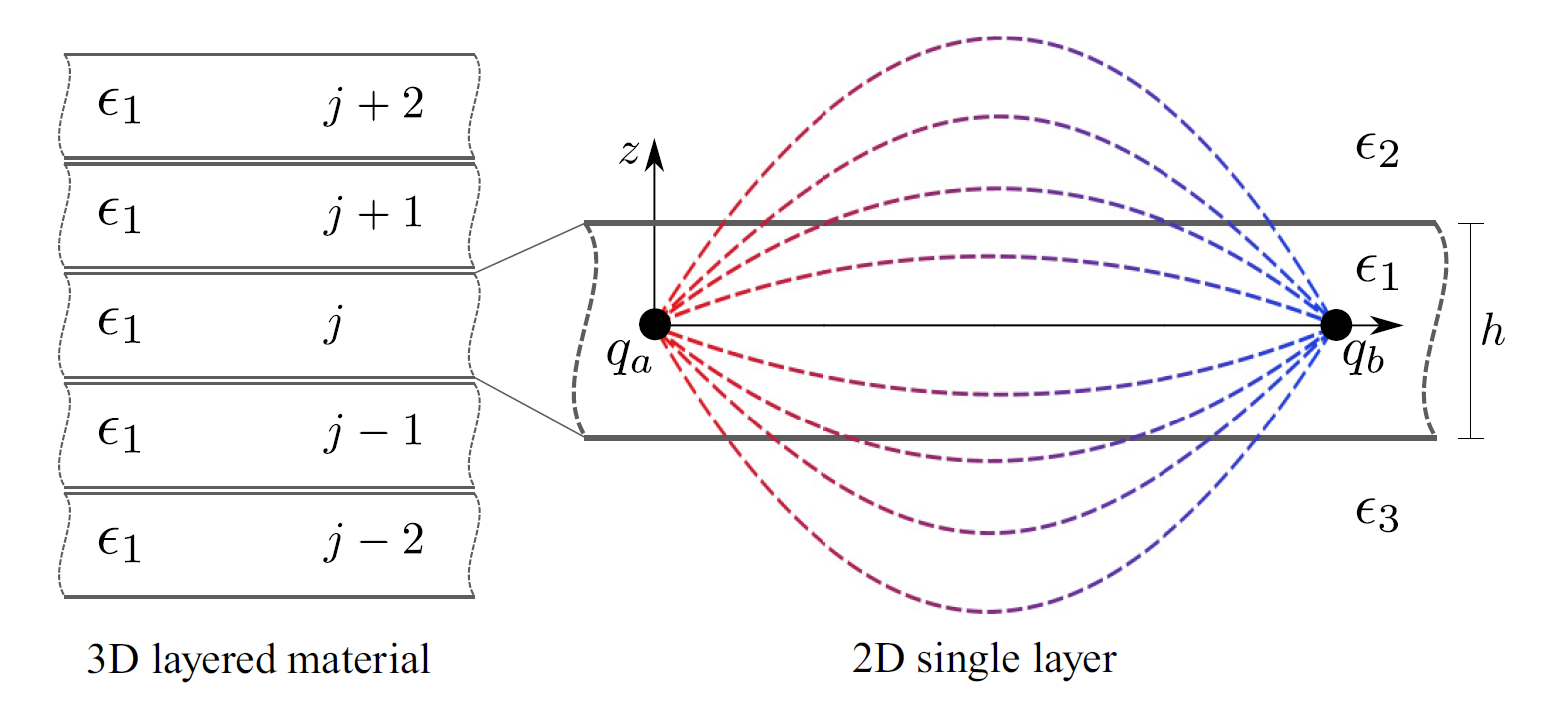
\includegraphics[width=.7\textwidth]{img/screening.PNG}
    \caption{Three-dimensional material consisting of several layers with thickness $h$ and dielectric constant $\epsilon_1$. The variables $\epsilon_2$ and $\epsilon_3$ are the dielectric constants of the slab between the layers. The dashed lines correspond to the electric field created by the two charges $q_a$ and $q_b$ \cite{Roesner2015} (image source: \textcite{Roesner2015}).}
    \label{fig:screened}
\end{figure}

Suppose one is dealing with a three-dimensional material with several identical layers which all have the same dielectric constant $\epsilon_1$ (see figure \ref{fig:screened}) \cite{Roesner2015}. The space between these layers is either filled with another dielectric material with constants $\epsilon_2$ and $\epsilon_3$ or simply empty space such that $\epsilon_2=\epsilon_3=\SI{1}{eV}$. Let $h$ be the thickness of one layer and $z$ the distance from the origin, such that that the dielectric materials can be written as (see figure \ref{fig:screened})
\begin{equation}
    \epsilon(z)=\begin{cases}\epsilon_2 &\iif z>\frac{h}{2}\\
    \epsilon_1 &\iif -\frac{h}{2}<z<\frac{h}{2}\\
    \epsilon_3 &\iif z<-\frac{h}{2}
    \end{cases}.
\end{equation}
Throughout the history of physics, starting with the French physicist Charles-Augustin de Coulomb (1736-1806), many different models have been proposed to properly represent the Coulomb interaction in real space. Some of them did not form proper divergence for in-plane separation at $r\to 0$ and others did not account for the surrounding environment in a correct way \cite{Cho2018}. In order to account for these effects, it is possible to use the following model \cite{Cho2018}
\begin{equation}\label{eq:cho}
\begin{split}
    U(\mathbf{r},\mathbf{r}'') \equiv U(r)&= \frac{e^2}{\epsilon_1 r} + 2\sum_{n=1}^\infty\frac{e^2L_{12}^nL^n_{13}}{\epsilon_1\sqrt{r^2+\brackets{2nh}^2}}\\
    &+ \brackets{L_{12}+L_{13}}\sum_{n=0}^\infty\frac{e^2L^n_{12}L^n_{13}}{\epsilon_1\sqrt{r^2+\brackets{\brackets{2n+1}h}^2}}\\
    &\with L_{1n}=\frac{\epsilon_1-\epsilon_n}{\epsilon_1+\epsilon_n},
\end{split}
\end{equation}
where $r=||\mathbf{r}-\mathbf{r}''||$ is the absolute distance. The first term represents the classical Coulomb interaction which is proportional to $1/r$, whereas the second and the third terms take the environmental screening with $\epsilon_2$ and $\epsilon_3$ into account \cite{Cho2018}. Nevertheless, ab initio data has shown that the on-site potential, where $r\to 0$, does in fact not diverge \cite{Goodwin2019}. This can be corrected with the Ohno potential fit, where 
\begin{equation}
    \rho = \sqrt{r^2+\delta^2}
\end{equation}
replaces $r$ in equation \ref{eq:cho} \cite{Goodwin2019}. $\delta>0$ is a constant which can be fitted such that the on-site potential ($r\to 0$) can be displayed with the screened Coulomb interaction $U(\rho)$. In other words, $U(\rho \to 0)$ will not diverge.

%%%%%%%%%%%%%%%%%%%%%%%%%%%%%%%%%%%

\subsection{Plasmonic Excitations}\label{plasmonic_excitations}

Plasmons can be examined by analysing the collective energy loss of electrons, which occurs when plasmonic excitations arise \cite{Bao2017}. This method is known as the electron energy loss spectroscopy (EELS), which can be derived from the dielectric function (see equation \ref{eq:dielectric}). The dielectric function itself can be calculated with the polarisability matrix and the Coulomb interaction matrix. The latter of these matrices will be determined with the use of data derived from first principles (ab initio data). This data will be created with the constrained random-phase approximation\footnote{The random-phase approximation (RPA, also referred to as the 'dynamical Lindhard approximation') assumes that electrons only respond to the total potential. As a consequence the exchange-correlation contribution is neglected and the polarisability and dielectric function depend on the variables $\mathbf{r},\mathbf{r}'$ and $\omega$ \cite{Girvin2019}. The constrained random-phase approximation (cRPA) refers to the RPA where
excitations between certain low-energy bands are neglected \cite{Vanhala2020}. That way we can investigate the effect of dielectric screening of substrates before applying the RPA. For more details on the RPA see chapters 15.7 and 15.8 in \textcite{Girvin2019}.}. This data will be used to find suitable parameters for the screened Coulomb interaction $U(r)$ (see equation \ref{eq:cho}), such that a continuous model can be derived. From this model we can create an interaction matrix $U_{i,j}$, such that together with the tight-binding Hamiltonian (see equation \ref{eq:hamil_coul_red}), the dielectric matrix can be found with the random-phase approximation (RPA). 

The dielectric function can be diagonalised to find eigenvalues and eigenvectors, i.e. \cite{Westerhout2021}
\begin{equation}
    \epsilon\brackets{\mathbf{r},\mathbf{r}',\omega}=\sum_n\epsilon_n(\omega)\ket{\phi_n(\omega)}\bra{\phi_n(\omega)},
\end{equation}
where $\epsilon_n(\omega)$ are the eigenvalues/eigenenergies and $\ket{\phi_n(\omega)} = \phi_n\brackets{\mathbf{r},\mathbf{r}',\omega}$ are their corresponding eigenmodes. The full EELS can be determined by finding the leading eigenvalue $\epsilon_1(\omega)$. In that case the EELS can be written as
\begin{equation}\label{eq:eels}
    \mathrm{EELS}(\omega)=-\im\brackets{\frac{1}{\epsilon_1(\omega)}},
\end{equation}
or equivalently
\begin{equation}
    \mathrm{EELS}(\omega)=\max\abrackets{-\im\brackets{\frac{1}{\epsilon_n(\omega)}}}.
\end{equation}
Mathematically, plasmons are defined as the eigenmodes $\phi_n\brackets{\mathbf{r},\mathbf{r}',\omega}$ corresponding to the frequencies, where
\begin{equation}
    \epsilon_1(\omega) = 0.
\end{equation}
We can immediately see why the EELS is a useful tool to find plasmons, as the peaks/maxima of the EELS correspond to $\epsilon_1(\omega) \to 0$. Nevertheless, these plasmon frequencies can also be found when determining the frequency at which $\re(\epsilon_1(\omega))=0$. The eigenmodes, which are the eigenvectors found during the diagonalisation of the dielectric matrix, represent the plasmons, which can now be portrayed in real-space.\medskip

To summarise, we first determine the matrix elements of the tight-binding Hamiltonian (see equations \ref{eq:hamil} and \ref{eq:reduced_hamil}), which we will denote as $H_\ttext{tb}$. Combining this matrix with a specified frequency range, we can determine the polarisability matrix $\Pi(\omega)$ (see equation \ref{eq:pi_damp}). At the same time we can make use of first principle calculations to derive the ab initio data. From this data we can fit the parameters for a continuous screened Coulomb potential $U(r)$ (see equation \ref{eq:cho}), which in turn can be converted to a Coulomb interaction matrix $U_{i,j}$. The dielectric function $\epsilon(\omega)$ (see equation \ref{eq:dielectric}) can then be determined with the RPA from the Coulomb interaction matrix elements $U_{i,j}$ and the polarisability $\Pi(\omega)$. Schematically this can be written as follows:

\begin{equation}
    \boxed{\begin{rcases}
    (H_\ttext{tb},\omega) &\Rightarrow \Pi(\omega)\\
    \text{cRPA} \Rightarrow \ttext{ab initio data} &\Rightarrow U(r) \Rightarrow U_{i,j}
    \end{rcases} (\Pi(\omega),U_{i,j}) \Rightarrow \text{RPA} \Rightarrow \epsilon(\omega) }
\end{equation}






\begin{comment}% Dispersion Relation
The so-called dispersion relation is given by the EELS with $\brackets{\mathbf{r},\mathbf{r}'}$- and frequency-dependency, such that \cite{Roesner2016,Groenewald2016}
\begin{equation}
    \mathrm{EELS}(\mathbf{q},\omega)=-\im\brackets{\frac{1}{\epsilon_m(\mathbf{q},\omega)}}.
\end{equation}
\end{comment}







